% Formatting questions:
%	Should all statistics (e.g., p-value, t-value, F-value) be in math environment? (e.g. $p$-value)
%	What about F(1, 50), 95\% CI [69, 420]? How much is math and how much is \mbox{}?
%	Ditto ~Normal, ~Cauchy, and their parameters. mbox? math?

% \citet{} is doing a bad thing by using \& in text
% (APA 6e style is to use ``and'' in text, \& in parenthesis)

% To do:
%	Let Jeff do his thing
%	Import tables from Excel into LaTeX? Or are we going to try to roll them w/in LaTeX?
%	I've been thinking it might be nice to have a graph of P(y|theta)

\documentclass[fignum,nobf,man]{apa}
\usepackage{apacite}
\usepackage{bm}
\usepackage{pcl}
\usepackage{graphicx}
%\usepackage{mathtools} %crashing for some reason
\usepackage[longnamesfirst]{natbib}
\usepackage[american]{babel}
%  Adding caption package in attempt to add `normal' table captions, too
%\usepackage{caption} % i don't think it's actually working, think we have package conflct
\usepackage{multirow}
\usepackage{pdfpages}

% Need better shortTitle
\rightheader{Bayesian Reanalysis of Violent Media}
\shorttitle{Bayesian Reanalysis of Violent Media}

\leftheader{Hilgard et al.}

\author{Joseph Hilgard, Christopher R. Engelhardt, Bruce D. Bartholow, and Jeffrey N. Rouder}
% Need better title
\title{A Bayesian Reanalysis of Studies in Violent Media Research}

\affiliation{University of Missouri}

\note{\begin{flushleft}

\vspace{1in}
Joseph Hilgard\\
jhilgard@gmail.com
\end{flushleft}
}

\abstract{Despite decades of research, the purported association between violent video games and aggressive outcomes remains controversial. One source of controversy stems from questions of experimental control, as advocates of the effect argue that the effect remains when stimuli are matched in all irrelevant dimensions, while detractors of the effect argue that the effect is eliminated under better-matched conditions. % Trying to improve this transition. 
Both these arguments require statistical evidence for the null hypothesis: advocates need to argue that confounding differences between games are zero, whereas skeptics need to argue that the effects of violent content are zero. This evidence cannot be provided by the use of null-hypothesis significance testing. To evaluate these claims, we apply a more appropriate Bayesian analysis to measure evidence for or against the null hypothesis. We conclude that small-sample pilot tests cannot rule out substantial confounds. Furthermore, we find that studies that claim to find an absence of violent video game effects vary substantially in the strength of evidence, with some even finding evidence of an effect. We recommend the use of Bayesian analyses, larger sample sizes, and the creation of custom-designed games for experimental research.}

\begin{document}
\maketitle

%\section*{Introduction} %I guess one of Jeff's style packages is preventing this from suppressing properly with \section*{}
Despite more than two decades of research, the scientific literature on whether violent video games cause aggressive outcomes remains divided and contentious. To date, this relationship has been examined in literally hundreds of studies as well as in aggregate by four different meta-analyses. Even the meta-analyses are divided and contentious---two argue that there is a meaningfully large effect \citep{Anderson:etal:2010,Greitemeyer:Mugge:2014} and two argue there is no meaningful effect \citep[e.g.,][]{Ferguson:Kilburn:2009,Sherry:2001}. % Chris comments re: "meaningfully large effect"
Note here that both positions, that video game violence increases aggression and that video game violence has no effect on aggression, are theoretically important and {\em a priori} plausible.  They both deserve serious consideration on an equal playing field.  

In this debate, a major point of contention has been the degree to which the observed effects instead may be caused by confounding game features other than violent content. When stimuli are appropriately matched on these features, it has been argued, the effect is eliminated. For example, \citet{Adachi:Willoughby:2011} argue that it is competition rather than violence that causes increases in aggressive behavior, and that matching game stimuli on competitive content eliminates the purported effect of violence. Similarly, \citet{Przybylski:etal:2014} argue that changes in aggressive affect may be due to difficult, competence-impeding controls rather than violent content. Finally,  \citet{Elson:etal:2013} argue that changes in aggressive behavior are caused by differences in pace of action rather than violent content. Each of these arguments favors the position that under certain circumstances there is no effect of video game violence on aggression.

Although the position that there is no video-game-violence effect is plausible and theoretically important, there is a difficult statistical problem in stating evidence for it. Null-hypothesis significance testing (NHST), the nearly ubiquitous approach for inference in this domain, %in research? in psychology? 
may not be used to state evidence for the null hypothesis that the true effect size is zero.  NHST may certainly be used to reject the null hypothesis in favor of an alternative hypothesis, thereby providing evidence for an effect, but it cannot reject the alternative hypothesis in favor of the null hypothesis. A $p$-value greater than .05 may reflect a true effect size of zero, but, alternatively, it also may reflect insufficient power to detect a true nonzero effect. Therefore, it is unknown whether the previously discussed null findings reflect a true null or a lack of power.    Needed is a method for stating positive evidence for the null rather than a lack of evidence for an effect. % "Needed is" seems too Yoda for me.

The importance of the null hypothesis in building theory has been understated in psychology though there are notable exceptions of researchers arguing for its critical importance \citep{Gallistel:2009,Rouder:etal:2009a}.  In the current context, whether there is or is not an effect has direct theoretical implications on how media influences affect, cognition, and even behavior.  Even proponents of video-game-violence effects have the need to state positive evidence for null hypotheses.  In all experiments there is a critical need to match features between violent and nonviolent games so that experimental control is maintained over all game features besides violence.  When these features are matched, it is argued that the violent and nonviolent game stimuli differ only in violent content, and so any observed differences in aggressive outcomes are caused by violent content alone and not by other confounding differences.  So crucial is this matching process that it has been deemed a necessary criterion of best-practices studies in some meta-analyses \citep{Anderson:etal:2010}.

In the present manuscript, we examine the strength of evidence for video game violence vs. a fairly-treated no-video-game violence null.  To do so, we present Bayesian inference which indeed allows researchers to state positive evidence for either hypothesis as determined by the data.  In the next section, we present these Bayesian methods and explain how they can be used not only to find evidence for effects of experimental factors, but also evidence for invariance in outcomes with respect to experimental factors.  % Too wordy? Could cut back to "can be used to find evidence for effects or for invariances"
Following this, we assess whether violent and nonviolent game stimuli appear to be well-matched by reanalyzing several pilot studies in violent video game research.  We then examine the strength of evidence of invariance in those studies reporting no significant effect of violent content.  Finally, results are summarized and practical suggestions offered for optimally informative research. % Gave it a shot.
% Jeff recommends providing a full outline of the paper here.
% Suggested order:
%	Bayes factors come immediately next,
%	then the folly of pilot testing
%	Null results (e.g. Adachi & Willoughby, Elson, Przybylski, Valadez &Ferguson)
%	then wrap it up with three cheers for Bayes, a call for larger samples, and a call for modified-game paradigms.

\section{Bayesian Inference}
At the heart of being able to state evidence for an effect or for an invariance is Bayesian model comparison.  Bayesian model comparison has a long history in statistics and even in psychology.  Perhaps the first to suggest the methods we cover was Laplace (1829, republished in 1986), and seminal development occurred through World War II and was presented most comprehensively by \citet{Jeffreys:1961}.  \citet{Edwards:etal:1963} were perhaps the first psychologists to recommend the approach and did so with uncommon gusto in their landmark {\em Psychological Review} article.  The method has gained increasing popularity in statistics and psychology \citep{Berger:1996,Gallistel:2009,Raftery:1995,Rouder:etal:2009a,Wagenmakers:2007} and is rapidly becoming widespread especially in cognitive domains. % Berger 1996 is undefined 
The main hurdle to adoption has often been the difficulty of computation and the unavailability of software \citep{Gallistel:2009}, but these hurdles have been largely removed with Morey and Rouder's (2014) BayesFactor library for the {\bf R} statistics language.

\nocite{Laplace:1986,Morey:Rouder:2014}

In Bayesian analysis probabilities are used to confer a degree of belief on events, parameters, and even theoretically important positions.  Analysts start with stated beliefs, and then update them rationally and optimally using Bayes' rule.  For updating beliefs about positions, we use the following form of Bayes rule:
\begin{equation}
\frac{Pr(H_0 | \mbox{Data})}{Pr(H_1 | \mbox{Data})} = \frac{Pr(\mbox{Data} | H_0)}{Pr(\mbox{Data} | H_1)} \times \frac{Pr(H_0)}{Pr (H_1)} 
\end{equation}
It is best to start with the term on the far right, $Pr(H_0)/Pr(H_1)$ which is called the {\em prior odds}.  This term describes the researcher's beliefs about the plausibility of the positions before collecting the data.  The term on the left, $Pr(H_0 | \mbox{Data})/Pr(H_1 | \mbox{Data})$, called the {\em posterior odds}, describes the researchers beliefs after collecting the data.   The key question is how did the data affect the beliefs, or, restated, what is the evidence from the data.  This evidence is described by the middle term,  $Pr(\mbox{Data} | H_0)/Pr(\mbox{Data} | H_1)$, whch is also called the {\em Bayes factor}.  We will denote the Bayes factor with $B$, and subscript it to indicate which hypothesis is in the numerator and denominator:
\[
B_{01} = \frac{Pr(\mbox{Data} | H_0)}{Pr(\mbox{Data} | H_1)} \mbox{ and } B_{10} = \frac{Pr(\mbox{Data} | H_1)}{Pr(\mbox{Data} | H_0)}.
\]
Bayes factor values range from 0 to $\infty$ and describe how much more probable the data is under one position than another.  For example, $B_{01}=10$ means that the null is ten times more probably than the alternative while $B_{01}=.1$ means that the alternative is ten times more probable than the null.  Infinite support for the null and alternative are obtained when $B_{01}=\infty$ and $B_{01}=0$, respectively.  A Bayes factor of $B_{01}=B_{10}=1$ expresses equivalency; the data do not discriminate at all among the positions.

One of the key properties of Bayes factors is that it describes changes in beliefs rather than beliefs themselves.  Consequently, two researchers may not agree about the plausibility of positions {\em a priori}, and, in this case, they will not agree about the posterior plausibility.  Nonetheless, they may agree about the Bayes factors, or the evidence from data.  Therefore, the Bayes factor is not dependent on these prior odds and serves as evidence regardless of beliefs about the initial plausibility of positions.  In our view, because Bayes factors describes evidence or change in belief rather than belief itself, it is an ideal statistic for scientific communication.  This property contrasts favorably with conventional significance testing which is about making decisions with long-term error rates controlled rather than about expressing evidence form data. 

The remaining task is defining what the probability of data is under a hypothesis.  We describe the simple case where the data are normally distributed and the question is whether the true effect size is zero or nonzero.  The generalization to more complex cases is straightforward and will be discussed briefly thereafter.  Let $\delta$ and $\hat{\delta}$ describe a true or theoretical effect size and an observed effect size, respectively.  There are two probabilities that need to be computed,   $Pr(\mbox{Data} | H_0)$ and $Pr(\mbox{Data} | H_1)$.   The former is straightforward.  For this simple case, $Pr(\mbox{Data} | H_0)$ is $Pr(\hat{\delta} \mid \delta=0)$, which is obtained from the $t$ distribution.  Figure~\ref{BFfig}A shows the hypothesis that $\delta=0$ as an arrow at zero.  Figure~\ref{BFfig}B shows the probability density under this hypothesis for all values of $\hat{\delta}$ for a sample size of 40 observations divided evenly across two cells.  %Changing this to two-sample tests, as is the design typically  observed in this literature.
The case for the alternative is more complicated.  If the alternative is a single point, say $\delta=.2$, then it is relatively straightforward to compute the probability $Pr(\hat{\delta} \mid \delta=.2)$, which is obtained from a noncentral $T$ distribution.   This alternative too is represented as an arrow in Figure~\ref{BFfig}A and the probability density under this alternative is also shown in Figure~\ref{BFfig}B. The Bayes factor is simply the ratio of the probabilities.  So, for example, if the observed effect size is .4, as shown by the circles in Figure~\ref{BFfig}B, then the probability density for $H_0$ is 0.18, the probability density for $H_1$ is 0.32, and the Bayes factor $B_{01}$, the ratio is 1.8. % The Bayes factor B01, the ratio... weird comma?

The specification of a point alternative, though often done in power analyses, strikes us as too constrained.  In Bayesian analysis, the analyst can consider a range of alternatives.  Figure~\ref{BFfig}C shows the point null and a distributed alternative.  Under this alternative, smaller effects are more weighted than larger ones, and positive effects are as weighted as negative ones.  The shown alternative is the default one recommended by Rouder and Morey and colleagues \citep{Rouder:etal:2009a,Morey:Rouder:2011,Rouder:Morey:2012,Rouder:etal:2012} as being broadly appropriate for research in psychological sciences.  The probability density under this alternative for all values of $\hat{\delta}$ is shown in Fiugre~\ref{BFfig}D, and the density is more diffuse than that for the null.   As before, Bayes factor values are computed as the ratio of these probability densities.   Figure~\ref{BFfig}E shows Bayes factor values for the null vs. the Rouder-Morey default as a function of observed effect size. As can be seen, small observed effect sizes correspond to evidence for the null while larger values correspond to increased evidence for the alternative.  

%(JOE, I didnt touch the following paragraph, you can keep, rewrite, or delete)
% Maybe this would make for a good Figure X.F.
It is also possible to specify and compare more than one alternative hypothesis. This approach can be useful when two competing hypotheses would predict effects of different magnitudes or directions. It is also helpful when assessing the results of a replication: one alternative hypothesis can broadly describe the anticipated effect, while another alternative hypothesis can specifically describe the effect as obtained in previous research \citep[see][for an example]{Boekel:etal:2014}. %(See Boekel et al. (in press) for an example.) % Will the postfix render correctly?  
For an accessible introduction to the practice of specifying an alternative hypothesis and appropriate software tools, we suggest the interested reader consult recent work by \citet{Dienes:2011,Dienes:2014} and by \citet{Rouder:Morey:2012} and \citet{Rouder:etal:2012}.

\section{Arguing the Null in Pilot Testing of Matched Stimuli}
We apply the above approach to interpreting the results of stimulus-matching pilot testing.  Suppose we are designing a study to see whether violent content in games influences aggressive behavior. Participants will play one of two games (violent or nonviolent) and then have an opportunity to aggress against a confederate. In order to make a causal statement that the observed effects, if any, are specifically due to violence, it is useful to first make sure that the two games are alike in all dimensions save violence. We run a small pilot study ($n = 20$), asking each participant to rate each game for violence, difficulty, arousal, and enjoyment. Performing paired-samples $t$-tests on each outcome, only violence is found to significantly differ, $p < .05$. We might be tempted to conclude, then, that the two games are matched on the other outcomes. However, this conclusion does not follow on the basis of $p > .05$ alone.

In the research literature on violent games, advocates have suggested that this process of matching is one of the criteria that separate ``best practices'' studies that find larger effects from ``not best practices'' studies that find smaller effects \citep{Anderson:etal:2010}. At the same time, skeptics have suggested that matching games on certain dimensions eliminates the effect of violent games \citep{Adachi:Willoughby:2011}. However, interpretation of these pilot tests has been improper and incoherent. For example, pilot tests in this research domain have sometimes estimated the differences between stimuli as being large, but because the results were not statistically significant, the null hypothesis was considered confirmed. In one particularly remarkable case, post-hoc Bonferroni correction for multiple comparisons was applied to control the Type I error rate across comparisons on 14 dimensions, lowering the critical value of $p$ to .0036 \citep{Arriaga:etal:2008}. Differences as large as $r = .53$ were observed but not considered statistically significant due to the small sample size and harsh multiple comparison correction. To their credit, the authors acknowledge that the pilot sample was small, but still do not entertain the possibility that the pilot test provided evidence of differences; instead, they conclude that the pilot test indicates that the games are relatively well-matched.

The null hypothesis in such pilot tests cannot be supported by use of NHST because they are constructed so that the researcher is on the wrong side of the null hypothesis: trying to demonstrate the truth of the null with a statistical method that can only reject the null. Worse, the more data that is collected, the better the statistical power to detect a confound, and the more likely it becomes that one or more confounds will emerge as significant. This inferential approach, then, will reward researchers for collecting insufficient data and risks failing to detect substantial confounds. Indeed, with a sufficiently small pilot and harsh enough multiple comparison corrections, even large confounds will go undetected.

% A reader of an early draft asked me to put this early so that he would stop thinking "Why not use effect sizes and confidence intervals?" through the whole paper.
% I have moved it, for now, to the bottom of our Bayes subsection, without making edits for transition.
\subsection{Providing evidence for the null hypothesis}
% or Imperfect alternatives to nil-hypothesis NHST
Two alternatives to nil-hypothesis NHST come to mind. First, one could perform a significance test against a second null hypothesis of some effect. For example, when failing to detect an anticipated effect, one could test against the expected effect size $\delta$ with the secondary null hypothesis $H_{02}: \mu_1 - \mu_2 = \delta$. If the study retains $H_0$ while rejecting $H_{02}$, it could be argued that the study data are sufficiently unlikely given that the true effect size is $\delta$ \citep[e.g.,][]{Simonsohn:etal:2014}. However, this approach does suffer from the typical NHST problem of dichotomous inferences. Dichotomous NHST procedures cannot discriminate between no evidence, a little evidence, and a lot of evidence, instead concluding simply either that there is evidence or that there is not yet evidence. The problems of this dichotomization are particularly salient when one considers how slight changes in $p$-value lead to opposite conclusions, such as how the null is rejected at $p = .049$ but the null is retained at $p = .051$. NHST also cannot handle small amounts of evidence well. Given slight evidence, either the null is retained and the slight evidence is mislabeled as no evidence at all, or the null is rejected and the effect size is grossly misestimated. 

A second alternative is to instead quantify the effect size and its confidence interval (ESCI). This does have the advantage relative to NHST of being continuous in quantification.  However, ESCI provides neither quantifiable nor inferentially consistent statistics \citep[see][]{Morey:etal:2014}, and when making inferences using ESCI, researchers seem to mentally convert them to NHST anyway \citep{Hoekstra:etal:2014}. While it is true that values near the ends of the confidence interval are less likely, one cannot know exactly how much less likely they are. Similarly, a wide CI indicates that more samples would be necessary to provide a more precise estimate of the effect size, but at what point does the CI become sufficiently precise for inference? ESCI is, in our opinion, a useful descriptive tool, but does not permit inferences about the strength of evidence.

\section{Bayesian Analysis in Pilot Testing}
Because Bayesian analysis can provide positive evidence for the null hypothesis of no effect, it permits fair and appropriate tests of whether stimuli are matched. To test whether two stimuli are matched, one compares a null hypothesis of no difference ($H_0: \delta{} = 0$) and an alternative hypothesis of a moderate difference (e.g., $H_A: \delta{} \sim{} \mbox{Cauchy(scale = .5)}$). If it is unreasonable to expect that the stimuli are perfectly matched, a null hypothesis of minimal difference can be used instead to treat very small differences as practically equivalent to zero (e.g., $H_0: \delta{} \sim{} \mbox{Uniform(-.1, .1)}$, see the nullInterval argument for the ttestBF function in the BayesFactor {\bf R} package). 

Having specified these two hypotheses, the researcher conducts a pilot test. In this pilot test, participants rate the stimuli on all relevant dimensions.  The differences in ratings are quantified, and the probability of the observed differences given the null hypothesis and given the alternative hypothesis are compared. If the Bayes factor favors the null ($B_{01} > 1$), the researcher has evidence that the two stimuli do not differ on the particular dimension. If the Bayes factor favors the alternative ($B_{01} < 1$), this is evidence that the two stimuli do differ. Finally, if the Bayes factor favors neither hypothesis ($B_{01} \approx 1$), the data are not sufficient to discriminate between the two hypotheses.
 
Because uninformative data yields an uninformative Bayes factor while stronger data yields stronger Bayes factors, this approach to pilot-testing rewards researchers for collecting more, rather than less, pilot data. Again, this is preferable to an NHST approach, in which the desired $p > .05$ can almost always be obtained by collection of small, uninformative samples.  In the case that the resulting Bayes factor is not sufficiently compelling, the researcher may return to collect additional pilot data, as Bayes factors are not biased by conditional stopping rules \citep{Rouder:2014}. % Should there be a new paragraph starting here as I approach subjectivity in beliefs?
But how large must the Bayes factor be to be sufficiently compelling? Recall that posterior beliefs are the product of prior beliefs and the Bayes factor. In the case that two stimuli seem to be obviously matched, it may not be necessary to provide a lot of evidence in a thorough pilot test; in the case that two stimuli would seem to be poorly matched, substantially more thorough pilot testing will be necessary to demonstrate their matchedness.  There can be no objective threshold that separates ``sufficient evidence'' from ``insufficient evidence'', as prior beliefs are inherently subjective. %Consider removing scare quotes above?
Thus, to the question ``How much evidence do I need?'' the answer is simply ``Enough to convince your reviewers, readers, critics, and yourself.'' \citet[p. 12]{Rouder:etal:submitted} % 'submitted', or 2014? %Rouder, Morey, and Wagenmakers (submitted, p. 12) 
explain the value of evidence in the absence of a decision rule: 
\begin{quote}
Finely graded evidence may be thought of as a quantity, say like the weight of some number of bananas. If one has a pound of bananas, there is no reason to make a decision whether a pound is a significant weight of bananas. We may all agree that it is what it is, a pound, even though it may have different meanings to differently sized monkeys, say gorillas and spider monkeys. For a pound will satiate a spider monkey but not a gorilla, and so it is with evidence. We may all have our own thresholds but still agree a Bayes factor of 5 is a Bayes factor of 5, and in all cases it is half as much as a Bayes factor of 10 and twice as much as a Bayes factor of 2.5.
\end{quote}

The magnitude of the Bayes factor is not only influenced by the amount of data collected, but the parameters of the alternative and null hypotheses. When the alternative predicts very small effects, its predictions closely resemble those of the null hypothesis; thus, it can require large amounts of data to achieve the necessary precision to discriminate between the two hypotheses. Therefore, it may not be feasible to demonstrate that stimuli are matched to arbitrary precision via pilot testing.  Practical considerations of sample size may limit the degree of precision with which stimuli can be matched.

\subsection{Reanalysis of Select Pilot Tests in Violent Media Research}
To assess whether pilot tests have provided convincing evidence of the equivalence of matched game stimuli, we perform a Bayesian reanalysis of previous studies and assess the evidence for the null hypothesis. To compare the evidence for or against the null, we compare the null hypothesis of no difference $H_0: \delta \sim \mbox{Uniform(-0.1, 0.1)}$ 
against the alternative hypothesis of some difference $H_A: \delta \sim \mbox{Cauchy(scale = 0.5)}$. This choice of scale in the alternative hypothesis is subjective, but appropriate. Effects of violent games are expected to be small (e.g., $\rho = .21$, or about $\delta = 0.43$), so confounds should be examined on a similarly small scale. Increasing this scale variable will increase evidence for the null, while decreasing this scale variable will decrease the evidence for the null; this is because it is easy to demonstrate that there are not large effects, but difficult to demonstrate that there are not small effects. % Previous sentence: interesting clarification or needless digression?
We use the ttestBF function in the BayesFactor package \citep{Morey:Rouder:2014} to calculate paired-sample or two-sample Bayesian $t$-tests with scale on effect size set to 0.5 and a null interval over (-0.1, 0.1). By entering the sample size and the obtained $t$-value of each test, we calculate a Bayes factor describing the strength of evidence for or against the null.  
% Sub-subsections for each study? Or okay as ust individual paragraphs or two? Top paragraph okay where it is?

First, we re-examine pilot data from \citet{Arriaga:etal:2008}. Results are summarized in Table~\ref{ArriagaAndersonPilot}. The pilot test, with its sample of $n = 20$ (within subjects), has not provided strong evidence of matching between stimuli on all dimensions. Bayes factors reveal that there is evidence that some dimensions do not differ, but evidence that other dimensions do. After the pilot test, the readers and researchers %we? they?
are forty times more confident that the two games do not differ in involvement and three times more confident they do not differ in presence, boredom, satisfaction, identification, or excitement. However, they should also be twice as concerned that the games differ in feelings of competence, and four times as concerned that they differ in difficulty. These conclusions are very different from those of the original authors, who interpret the nonsignificant results of the pilot test as indicating that the games are equivalent on all measures, or at worst, that the results might be merely inconclusive. Given that the two tested video games, {\em Unreal Tournament} (a first-person shooter game) and {\em Motocross Madness} (a racing game), come from very different game genres with very different rules of play, and that the evidence indicates differences between games in competence and difficulty, we might not believe that the games are well matched.  It is possible, then, that the primary results from this study, in which the violent game was associated with greater aggressive behavior, %double-check this
are not caused by violent content specifically, but may be caused instead by experience of competence or difficulty of gameplay.
% Multiple comparisons footnote should go here:
\footnote{While this and other analyses in this section would seem to involve a problem of multiple comparisons, we remind the reader that Bayes factors express evidence, and that multiple comparisons problems are a matter of interpretation, not evidence. ``One should not confuse strength of evidence with the probability of obtaining it (Royall, 1997). Evidence is evidence even if, as one increases the circle of what tests are in the `family', the probability that some of the evidence will be misleading increases.'' (see Dienes, 2011, pp 280, as an excellent resource on this problem).}

Another classic pilot test in this literature is found in \citet[study 1]{Anderson:etal:2004}, in which 120 subjects each played one of 10 games (i.e, $n = 12$ per cell). The games {\em Glider Pro} and {\em Marathon 2} were selected as a matched pair differing in violent content but not in other dimensions. Our reanalysis is summarized in Table~\ref{ArriagaAndersonPilot}. Evidence for the null hypothesis is slight, and reanalysis indicates that the games instead may differ in amount of action. Because we obtain different $p$-values than the original authors, it is possible that our re-analysis based on summary statistics is yielding slightly different $t$-values than the authors' analysis based on the original data. One such source of reanalytic imprecision is that single-cell SDs are not available, and so variance had to be approximated with the reported mean squared error. This may cause us to over-estimate or under-estimate the SD of a particular cell. In any condition, the Bayes factor is not likely to change by much, and at this small sample size per cell, will not strongly favor one hypothesis over the other. Further data collection would be necessary to demonstrate the equivalence of these two games on these dimensions. % a lot of hemming and hawing in this paragraph.

Improper inferences regarding the results of pilot testing are also found among skeptics of violent media effects. We re-evaluate the pilot test from \citet{Valadez:Ferguson:2012}. This study used a three-factor one-way ANOVA design to compare a violent game condition to two non-violent game control conditions. In the violent game condition, participants played a segment from the later stages of the open-world shooter game {\em Red Dead Redemption}. In one control conditon, participants played a segment from the beginning of {\em Red Dead Redemption}, argued to contain little or no violence because of the early stage of the game, and in the other control condition, participants played the soccer game {\em FIFA}, a nonviolent game. Only a small sample was collected (cell $n$s = 15, 10, and 15, respectively, between-subjects), to rate each game on difficulty, competitiveness, and pace of action. Differences in difficulty and competitiveness were reported as not significant, $F(2,40) = 2.36, p > .05$ and $F(2, 40) = 3.09, p > .05$, respectively, while differences in pace of action were significant $F(2, 40) = 4.27, p = .02$. This last variable was explored through Bonferroni post-hoc analysis, and it was decided that the two control conditions differed from each other but not from the active condition. 

To determine the strength of evidence for or against invariance, we perform all pairwise $t$-tests, then convert these into Bayes factors. Results are summarized in Table~\ref{ValadezFergusonPilot}. Contrary to the author's conclusions, the results of the pilot test indicate that the games are not well matched. In particular, Bayes factors indicate evidence that the two {\em Red Dead Redemption} conditions differ in Competitiveness and the two control conditions differ in all dimensions. Most other comparisons are largely uninformative, as might be expected of the very small sample size. Given our prior beliefs that the early stages of a game are often rather easier than the later stages, that {\em Red Dead Redemption} and {\em FIFA} are very different genres of game, and that the evidence indicates differences between the conditions, we are again not convinced that the stimuli are well-matched. Rather than demonstrate that the stimuli are matched, the pilot test has instead indicated that the games are probably quite different. %Even large effect size estimates and modest amounts of evidence can result in nonsignificant p-values.

Some pilot studies are more successful in finding evidence of invariance. \citet{Adachi:Willoughby:2011} report two pilot studies intended to demonstrate that the games used ({\em Conan}, an action-adventure combat game, and {\em Fuel}, a racing game) were matched on certain game dimensions but differed in violent content. In the first pilot, $n = 14$ participants played each of two games (within-subjects). This pilot provided modest evidence that the two games did not differ in competition, difficulty, or pace of action, $B_{01}$s = 3.36, 3.12, and 2.68 in favor of the null, respectively. The subsequent Study 1 provided further slight evidence that the games did not differ, $B_{01}$s = 3.04, 1.07, and 2.24 in favor of the null, respectively. ($B_{01}$ = 1.07 is however no evidence one way or the other.) Whether this is sufficient evidence of matching is a subjective question. Considering that the two games came from very different genres (action-adventure, racing), it might not be sufficient to convince everyone that the games are identical in all ways besides violent content. Still, at least the pilot test did not indicate that the games instead differed. Note also that neither this study nor \citet{Valadez:Ferguson:2012} tested games for equivalence in frustration, so it is possible that other confounds exist but were not tested.

\subsection{Summary}
Because NHST cannot provide evidence in favor of the null hypothesis, it is inappropriate to argue that two experimental stimuli are matched on the basis of a non-significant test result.  Non-significant test results can almost always be obtained, even if the null hypothesis is false, through collection of an arbitrarily small sample size and application of harsh post-hoc corrections. 

Because of the inferential flaws of this approach and the historically small sample sizes used in previous pilot tests, we would not advocate the use of a pilot test as a best-practice criterion in meta-analyzing previous research literature \citep[c.f.]{Anderson:etal:2010}. As has been demonstrated above, pilot tests from this literature often provide little-to-no evidence that stimuli are matched, and in fact, often indicate that the two stimuli involve some confounds. Future research studies may be able to use larger pilot studies and provide better evidence of matching, but the evidence in the previous literature is not strong. % Important dig at Anderson et al., but where to put it?
 
As an alternative to NHST, we advocate the use of Bayesian statistics. Evidence presented this way can favor the null hypothesis of no difference, an alternative hypothesis of a confounding difference, or indicate an absence of evidence for either hypothesis. Researchers are rewarded for more thorough pilot testing by larger Bayes factors that indicate stronger evidence. These principles apply also to tests of primary hypotheses, as we explore next.

\section{Interpreting Null Results in the Violent Games Literature}
The controversy in this research literature has been caused, in part, by differences in study results across researchers. Some researchers report finding statistically significant effects of game violence, while other researchers report retaining the null hypothesis. Researchers who retain the null hypothesis often consider such a retention as indicating the absence of a true effect \citep[e.g.,][]{Adachi:Willoughby:2011,Elson:etal:2013,Ferguson:Rueda:2010,Valadez:Ferguson:2012}. In some particularly interesting studies, it is argued that the effect has been eliminated through improved experimental controls. Such research suggests that previous studies have overestimated the effect of violent media by mistaking the effects of confounding game features for the effect of violence. If true, this would indicate that effect size estimates from previous meta-analyses \citep[e.g., $r = .21$,][]{Anderson:etal:2010} are in error. Proposed confounds include competition \citep{Adachi:Willoughby:2011}, frustrated needs for competency \citep{Przybylski:etal:2014}, or pace of action \citep{Elson:etal:2014}. Research exploring these confounds has found significant effects of the confound but nonsignificant effects of violent content. 

These nonsignificant results do not necessarily provide evidence for the null hypothesis. In many of these studies, sample sizes have been small, and so the power to detect the theorized effect of violence has been poor.  For example, two experiments are reported by \citet{Adachi:Willoughby:2011} with total samples of $n = 40$ and $n = 60$. Other experiments are reported by \citet{Ferguson:etal:2008}, \citet{Ferguson:Rueda:2010}, and \citet{Valadez:Ferguson:2012} with sample sizes of $n = 50$ (at least, for subjects randomly assigned), $n = 77$, and $n = 100$, respectively. \citet[(Studies 1, 2, and 5)]{Przybylski:etal:2014} %bad parentheses
perform three experiments with $n = 100$, $n = 100$, and $n = 109$. Another study is reported by \citet{Elson:etal:2014} with a sample size of $ n = 80 $. Assuming that the true effect size of violent content on aggressive behavior is $ r = .21 $ as reported in Anderson et al.'s meta-analysis, these studies are underpowered. Sample sizes of 40, 60, 80, and 100 would yield one-tailed test power of 38\%, 50\%, 60\%, and 69\%, respectively (but note that for a larger effect, such as the expected effect on aggressive affect, $r = .29$, one-tailed power would be 59\%, 75\%, 85\%, and 91\%). An ESCI inspection of these studies (Table ~\ref{mainStudyResults}) indicates that many CIs are quite broad, and that many enclose both $ r = 0 $ and $ r = .21 $, suggesting that the data are insufficiently precise to favor one hypothesis over the other. 
%Cut materials from this paragraph: %However, we nevertheless would like to understand just how much evidence is in each of these studies so that we can assess the validity of the arguments. Because few of these studies use the same paradigm, and many apply new paradigms argued to have eliminated the effect through innovations in experimental control, we cannot combine and meta-analyze studies for greater power. Thus, these single samples of <80\% power each are all the evidence that is available for making an inference.

%Is this paragraph below too mean? We've all said stupid things about statistics in 2008 and 2011.
Because these samples are small and the tests underpowered, failure to reject the null may not provide evidence of the truth of the null.  This possibility is sometimes dismissed out of hand by authors. For example, \citet{Adachi:Willoughby:2011} argue that sample size is not important, saying that ``the effect size for game in the current study was zero (partial $\eta^2$ = .000), and thus increasing the sample size would not have made the effect statistically significant.'' (pp 266).  On the contrary, the effect size is measured with error, especially in small samples; increasing the sample size would not only increase the precision of measurement, but also could cause the estimated effect size to change substantially. A similar argument is advanced by \citet{Ferguson:etal:2008} % Why is BibTeX printing his first initials? Don't do that!! % I think it's trying to keep him straight from some other Ferguson? %Where'd the page number go??
``Although the null hypothesis can not traditionally be accepted as `true,' [Loftus (1996) presented that] if the 95\% confidence interval in group difference scores (e.g., $\mu_1 – \mu_2$) is reasonably small, the null hypothesis can be effectively accepted as true. Similarly, [Cohen (1994) suggested examining the confidence interval around the effect size.] Effect-size confidence intervals that cross zero effect can be reasonably concluded to be ‘untrue' and, thus, support the null.''  % bracketed sections may be replaced with \ldots
This approaches an ESCI understanding of the null, arguing that as more data is collected, larger effect sizes can be excluded as being comparatively unlikely. However, given that the effect size confidence interval in that manuscript extended to values greater than the meta-analytic estimate (95\% CI on $r = [-.26, 30]$), it does not appear that the 95\% confidence interval is ``reasonably small'' enough to reject the alternative hypothesis in favor of the null.

In some cases, the estimated effect size may be very close to that predicted by meta-analysis but the null hypothesis is retained by hundredths of a $p$-value. Does such an outcome provide evidence for the null hypothesis? For example, one of the study outcomes reported by \citet{Elson:etal:2013} only barely missed statistical significance, $p = .073$. Considering that the observed effect size on this measure ($r = .20$) closely approximated that reported in meta-analysis \citep[$r = .21$,][]{Anderson:etal:2010}, it does not seem appropriate to consider this a refutation of the effect. %As the saying goes, ``Surely God loves the .06 nearly as much as the .05'' \citep{Rosnow:Rosenthal:1989}. % cutting this, it's trite and Rosnow & Rosenthal have already been cited plenty.
Instead, it seems likely that this study provides some evidence for the effect, even if this evidence is not sufficiently strong to be considered ``significant'' by NHST. 

\subsection{Bayesian Model Comparison and Hypothesis Formulation}
To assess the strength of evidence for or against the null hypothesis, we re-evaluate these null findings through Bayesian model comparison. We now describe the models to be compared. First, there is the point-null hypothesis, which describes the true effect size as exactly zero: $H_0: \delta = 0$. Next, we specify two alternative hypotheses, one representing a broad hypothesis and one representing a very specific hypothesis. First, the broad hypothesis is that the true effect is probably small-to-medium in magnitude. We will refer to this minimally-informative alternate hypothesis as $H_{A1}$, the first alternative hypothesis, and model it with a minimally-informative JZS Prior. $H_{A1}$ thereby summarizes this hypothesis's predictions about the effect as a Cauchy distribution centered at 0 with a narrow width.
\begin{equation}
H_{A1}: \delta{} \sim{} Cauchy(scale = .4) 
\end{equation}
By evaluating the probability of this hypothesis relative to the null hypothesis, we create Bayes factor $B_{01}$, the probability ratio of $H_0$ as compared to $H_{A1}$. %As before, when effect sizes are large and have good precision, the data are increasingly improbable given the null relative to the, and the Bayes factor favors this alternative hypothesis, indicating evidence for an effect of small magnitude and nonspecific direction. When effect sizes are near zero, the data are relatively more probable given the null, and the Bayes factor favors the null over this alternative, indicating evidence for no effect. 
Second, the more precise hypothesis is that the true effect is equal to that estimated by previous meta-analysis, e.g. $r = .21 [.17, .25]$ \citep{Anderson:etal:2010}.  We use the meta-analytic effect size estimate and standard error to derive our second alternative hypothesis,
\begin{equation}
H_{A2}: \rho{} \sim{} Normal(mean=.21, sd=.02)
\end{equation}
By again comparing the probability of the data given $H_0$ against the probability given $H_{A2}$, we create Bayes factor $B_{02}$. $BF_{02}$ gives the measure of evidence for the null hypothesis relative to the meta-analytic expectation of the effect size. (Note that the mean and standard deviation used in $H_{A2}$ will vary depending on the particular outcome tested: aggressive cognition, aggressive behavior, and aggressive affect each have slightly different meta-analytic effect size estimates. Displayed above is $H_{A2}$ for the effect of violent game content on aggressive behavior.) %For these normally distributed effects, Bayes factors can be easily calculated with the online calculator provided by Dienes  (http://www.lifesci.sussex.ac.uk/home/Zoltan\_Dienes/inference/Bayes.htm). 

With these Bayes factors, researchers can now evaluate an experiment's results as supporting any of these hypotheses relative to each other. %either $H_0$ or $H_{A2}$.
If $B_{02} < 1$, the results replicate and support the meta-analytic findings. If $B_{02} > 1$, the results provide evidence for the null hypothesis, indicating that the null is more likely than the meta-analytic alternative, given the observed data.  Comparisons between $H_{A1}$ and $H_0$ or $H_{A1}$ and $H_{A2}$ could indicate evidence for an effect of a magnitude or direction not predicted by $H_{A2}$. This model comparison between the null and meta-analytic alternative is applicable in many research contexts in which researchers explore the mediators, boundaries, or potential confounds associated with a psychological phenomenon.

\subsection{Reanalysis of Null Findings in VVG Research}
We apply this approach to the current literature of studies claimed to have found evidence of no effect of violent video games on aggressive behavior. Each study has a confidence interval that overlaps with $r = 0$, which caused researchers to retain the null hypothesis and argue evidence for it. However, how much quantifiable evidence do these studies provide for the null, if any?

Findings are summarized in Table~\ref{mainStudyResults}. We find that, among these null findings, the strength of evidence for the null varies substantially. In studies with small sample sizes (Ferguson et al., Study 1; Adachi \& Willoughby, 2011, Study 1 and 2), %Not sure how the syntax works with several prefixes and several studies within a single \citep{} call
evidence for the null in each experiment is slight. This indicates that the evidence provided by Adachi and Willoughby does favor the null hypothesis of no effect, but that a third, larger experiment might be conducted before we conclude that there is no effect of violent content on aggressive behavior so long as competitive content is matched. % save the previous sentence for discussion section?
In studies with larger sample sizes (Ivory \& Kalyanaraman, 2007, aggressive cognition; Przybylski et al., 2014, Study 1, 2, and 5; Tear \& Nielsen, 2014), %same deal here re: citep with multiple prefixes
evidence for the null is much stronger.	Finally, in cases where effect sizes were close to r = .21 but the confidence interval failed to exclude zero, we do not interpret the study as disproving $H_{A2}$ in favor of $H_0$. Bayes factors recognize that $r = .20$ much more closely resembles $r = .21$ than it does $r = .00$. Thus, re-examination of the effect of violent game content on noise intensity in \citet{Elson:etal:2013} indicates a moderately informative replication. The non-significant result has been misinterpreted as support for the null when instead support has been found for the alternative.

A similar phenomenon is observed in \citet{Valadez:Ferguson:2012}. 
In this study, participants' hostile feelings were measured before and after playing one of three games: a late-game section of {\em Red Dead Redemption} (the active condition), an early-game section of {\em Red Dead Redemption} (one control condition), and {\em FIFA} (a second control condition). %end potentially redundant portion
%Participants played the game for either 15 or 45 minutes. 
The condition in which the participants played the beginning section of {\em Red Dead Redemption} was considered a nonviolent control condition, as was {\em FIFA}. Thus, the latter section of {\em Red Dead Redemption} was compared to the other two conditions, and with a time (pre-, post) X game (active, controls 1 \& 2) test statistic of $F(1, 94) = 3.11, p = .09, r = .17$, the authors argued positive evidence for the null hypothesis. On the contrary, compared to the meta-analytic estimate of the effects of violent games on aggressive affect ($r = .29, [.25, .34]$, \citet{Anderson:etal:2010}) %the formatting here is fucked up
, the data slightly support the alternative hypothesis, not the null, at 1-to-1.9 odds. 

% Having a little trouble writing the appropriate transition sentence into this section
There is another issue with this study that requires reanalysis. It seems unlikely that the early section of {\em Red Dead Redemption} was truly nonviolent. Inspection of game footage indicates that the player-character is shot in a scripted scene within the first 15 minutes of play (see http://youtu.be/3lAB1JlbVIM?t=5m28s). This control condition therefore may better represent an active violent-game condition.  Thus, we performed the analysis again, this time comparing the two {\em Red Dead Redemption} conditions against the {\em FIFA} condition. This yields an effect size of $r = .22, [.02, .39]$  with  $B_{02}$ of 1-to-8.54, indicating fairly strong support for the meta-analytic alternative. However, this effect must be considered in light of an overall decrease in aggressive affect across all conditions from pretest to posttest, $F(1, 94) = 8.15, p = .005, r = .28 [.08, .44], B_{01}$ = 1-to-7.7 in favor of the nonspecific alternative. Thus, while this study provides evidence that violent games increase aggressive affect relative to nonviolent games, it also suggests that this observation is not due to increases in aggressive affect as a result of violent gameplay, but rather, smaller decreases in aggressive affect relative to those caused by nonviolent gameplay. (However, remember also that the conditions do not appear to be well-matched, and so this phenomenon could still be due to the same confounds that are suspected to cause the effect observed in other research.) Future research could explore this possibility through application of repeated measures designs, but be aware that repeated measurement of aggressive outcomes immediately before and after violent gameplay may alert participants to the research hypotheses and invalidate the study results. 

In summary, while all nonsignificant findings receive the same decision in NHST, a Bayesian analysis provides a more nuanced perspective by providing a quantification of continuous amounts of evidence. Attention to the strength of evidence will help researchers to determine whether they have evidence of no effect, evidence of an effect, or inconclusive evidence. This evidence tells researchers whether a research finding has been replicated, an effect has been disconfirmed, or a boundary of the phenomenon has been reached.

\subsection{Still No Replacement for Data Integrity} %Subsection?
We describe above how \citet{Elson:etal:2013} seem to have found evidence for the theorized effect despite an original argument for the null based on $p > .05$. In correspondence with these authors, they asked that we consider their criticism that the Competitive Reaction Time Task measure of aggression %(citation needed?) 
used is flexibly quantified, potentially allowing researchers to selectively report the quantification with the biggest effect size or the smallest $p$-value \citep{Elson:etal:2014}. In this literature, they argue, this particular measure is quantified in many different ways across studies, suggesting that researchers may attempt several different quantifications until one yields statistical significance. These concerns about flexible analysis apply also to Bayesian analyses, as Bayes factors are still a function of the data and thus still sensitive to flexibility in quantification. \citet{Elson:etal:2014} demonstrated that the same experiment can yield substantially various effect sizes and p-values depending on which quantification strategy is used. In the same way, the obtained $B_{02}$ varies substantially depending on the quantification: if mean intensity is used, $B_{02}$ favors the alternative, 1-to-5, but if mean duration is used, $B_{02}$ favors neither hypothesis, 1-to-1. We examine these fluctuations in Bayes factor across quantification strategy in Table~\ref{ElsonCRTTHacking}.  As \citet{Elson:etal:2014} had noticed, various quantification strategies yielded effect sizes ranging from $\omega = -.32$ (count of low-volume trials, here reported as negative, as it is in the direction opposite to that hypothesized) to $\omega = .00$ (first-trial volume) to $\omega = .39$ (count of high-volume trials). Similarly, $BF_{02}$ ranges from 1400-to-1 (count of low-volume trials) to 3.52-to-1 (first-trial volume) to 1-to-280 (count of high-volume trials). To minimize potential flexibility in quantification, we suggest that researchers preregister their analyses, share the raw task data, or provide evidence of the validity of a particular quantification, when possible. %Several of these goals can be facilitated by third-party services such as the Open Science Framework. % Third option is really cause for a whole set of studies...

\subsection{Summary}
Clearly, $p > .05$ can describe a wide variety of situations, and thus, its inferential value is limited. Among the articles reviewed in this section, $p > .05$ applied to a range of all possible study results: some studies had strong evidence for the null, others had only slight evidence for the null, and still others actually supported the alternative. As in the pilot testing example above, failure to reject the null does not constitute evidence for the null and may instead represent insufficient sample size. Even when sample sizes are sufficient, there still remains the issue of quantifying the evidence for or against the null. This can be accomplished by the application of Bayesian model comparison techniques presented by \citet{Rouder:Morey:2012, Rouder:etal:2012}
and \citet{Dienes:2011, Dienes:2014}. %These techniques can be used to perform a full 2x2 ANOVA, finding evidence for effects of certain factors while also finding evidence against effects of other factors, as appropriate.

Alternatives to Bayes factor exist, in that researchers can conduct hypothesis tests against an expected effect size or examine the obtained effect size and confidence interval, but these approaches are less informative than Bayesian model comparison. Applying a hypothesis test to see if the effect is significantly smaller than $r = .21$ would simply report that the data were incapable of rejecting either hypothesis, even though, as our analyses demonstrate, there is at least some evidence in many of these studies. One could instead attempt to interpret the ESCI, arguing that, because $r = .21$ is nearer the extremes of the interval, perhaps some of these studies provide some evidence for the null. However, in the absence of an explicitly defined alternative hypothesis %and a Bayesian analysis
, it is not possible to know how much evidence this represents, or even which hypothesis is supported.

Finally, Bayesian analysis is still a function of the data and cannot address concerns about selective reporting. Bayes factor represents the strength of reported evidence. When evidence is selectively reported according to the hypothesis it supports, Bayes factor will be biased. We urge researchers to pre-register their hypotheses and analytic strategies, including method of CRTT quantification. We further urge researchers to attempt a thorough and systematic validation of the CRTT in an attempt to choose a limited number of methods which clearly measure a limited number of constructs. Like any other statistical analysis, Bayesian model comparison is still subject to the problem of ``garbage in, garbage out.'' % Some of this now seems redundant with the sub-section's concluding sentence.

\section{Discussion} % Grand summary? Let's not have two "summary" headings next to each other.
Making principled and coherent arguments for the null hypothesis is a crucial part of the scientific process. In violent media research, the null hypothesis is frequently argued, first, in matching stimulus materials in pilot testing, and second, in demonstrating the boundary conditions or absence of an effect of violent media. Despite the importance and frequency of these endeavors, traditional statistical practices cannot support these goals. %P-values greater than a critical threshold do not have any interpretation as supporting the null hypothesis, as they only indicate an absence of evidence for an effect, not an evidence of absence of an effect.
As an alternative, we suggest Bayesian model comparison, which allows for fair and principled tests between the null hypothesis and a reasonable alternative hypothesis. % These Bayesian alternatives require the specification of a reasonable alternative hypothesis. Once researchers have specified an alternative hypothesis, this hypothesis can feasibly be falsified in favor of the null hypothesis. While specification of an alternative hypothesis may sound daunting, it is quite easy, and numerous resources exist to facilitate and evaluate the choice of an alternative hypothesis %(e.g., Dienes, 2011, 2014; Rouder et al., 2012). %appropriate citations? bear repeating?

Our re-analysis found that research in this area would benefit from larger samples and more finely-graded interpretations of results. Inspection of pilot studies found that many pilot studies provided little evidence of matching, and in some cases even provided evidence of confounding differences between game stimuli. In similar fashion, studies in this literature arguing no effect of violent game content were found to vary substantially in the strength of evidence for the null. In two cases, %Elson and... Ferguson 2008? Valadez&Ferguson?
a $p$-value very close to the critical threshold was presented as a disconfirmatory finding; re-evaluation of this report indicates instead modest support for the alternative hypothesis. We applaud and encourage research efforts in this area which strive to test the boundaries and causal substrates of the effects (if any) of violent games on aggressive thoughts, feelings, and behavior. However, it is clear from this review that some arguments would benefit from greater evidence. There is strong evidence that violent game contents do not seem to influence aggressive affect independently of player's experienced competence \citep{Przybylski:etal:2014}, but weaker evidence that games matched for competitive content do not influence aggressive behavior \citep{Adachi:Willoughby:2011}. Further direct or conceptual replications may be necessary before the evidence is sufficiently persuasive. 

We offer two other practical recommendations to improve pilot-testing and primary tests of hypotheses in this literature. First, we note that it may not be feasible to pilot test and match game stimuli to necessary precision. One could potentially invest many subjects in such a test only to find evidence that the games are not well matched. As an alternative to pilot testing commercially-available games for equivalence, we instead favor the approach of software modification. In this approach, researchers take an existing game and modify it with software tools so that the core game is the same, but the construct of interest varies across conditions. It is not unlike adjusting the parameters of computer task script. Because games developed in this way are more obviously matched, as the unmodified portions of the game's code are identical between versions, it requires less pilot evidence to conclude that they are indeed matched. One such manipulation, which involves identical game files which vary in violent content and in the difficulty of gameplay, has been made publicly available for use on OSF \citep{Hilgard:2014}. However, such homemade game modifications will have their limits. It will be infeasible to make professional-quality game modifications with graphics, gameplay, and acting on par with modern popular video games. While research suggests that graphical fidelity is not an important moderator of game effects \citep{Ivory:Kalyanaraman:2007}, it is possible that such homemade games do not capture the full real-world phenomenon of video gaming.

As a second practical recommendation, we ask that researchers collect larger samples in their experiments. Effects in this research domain are known to be small. Thus, large samples will be necessary to discriminate effectively between the null and alternative hypothesis. %To collect larger pilot samples, perhaps pilot tests could be conducted as an appendix to another experiment. 
It is possible that some effects are too small to be feasibly studied in single-institution experiments. Multi-site investigations could help to increase sample sizes. {\em Antagonistic} multi-site collaborations could be especially productive, having the additional benefit of reducing concerns of bias %or competence 
within individual research teams. %citation needed?

We close with an optimistic thought about how Bayesian analysis might further shape the scientific process. It is well understood that, historically, papers finding significant ($p < .05$) effects are more likely to be published than are papers without significant effects \citep{Cooper:etal:1997,Atkinson:etal:1982}. This process is thought to contribute to publication bias, in that only research finding an effect gets published, and questionable research practices, in that researchers muss with their results until the necessary $p < .05$ threshold is reached. Both of these processes will lead to overestimated effect sizes and the propagation of Type I errors. % Can this be argued? Dickersin et al 1987 argue that pub bias in clinical trials stem from lack of researcher, not publisher, interest. I'd say that in social psych it is clear that sig findings are more publishable, especially 10-20 years ago.
With Bayes factors, there is no such dichotomization or sufficient threshold; instead, evidence is collected and its strength reported. Acceptance of evidence as a continuous quantity may, we hope, reduce journals' and researchers' preference for results that just pass an arbitrary statistical threshold. By assessing the finely-quantified weight of evidence for each argument from each experiment, we can reach a greater understanding of what is certain, what is uncertain, where evidence is truly contradictory, and where we may simply have come to a misunderstanding.

% I like this sentence below but don't know if there's anyplace it still fits into the manuscript:
% This nuance is lost in NHST, which provides only dichotomous accept/reject decisions. It is perhaps this dichotomization of evidence which is, in part, responsible for the heated debate in the violent media literature, as each side may misunderstand their rejections or retentions of the null as decisive evidence for or against the effect. 

% % % % % % % % % % % % % % % %
% Hey guys, tables over here  %
% % % % % % % % % % % % % % % %

\begin{figure}
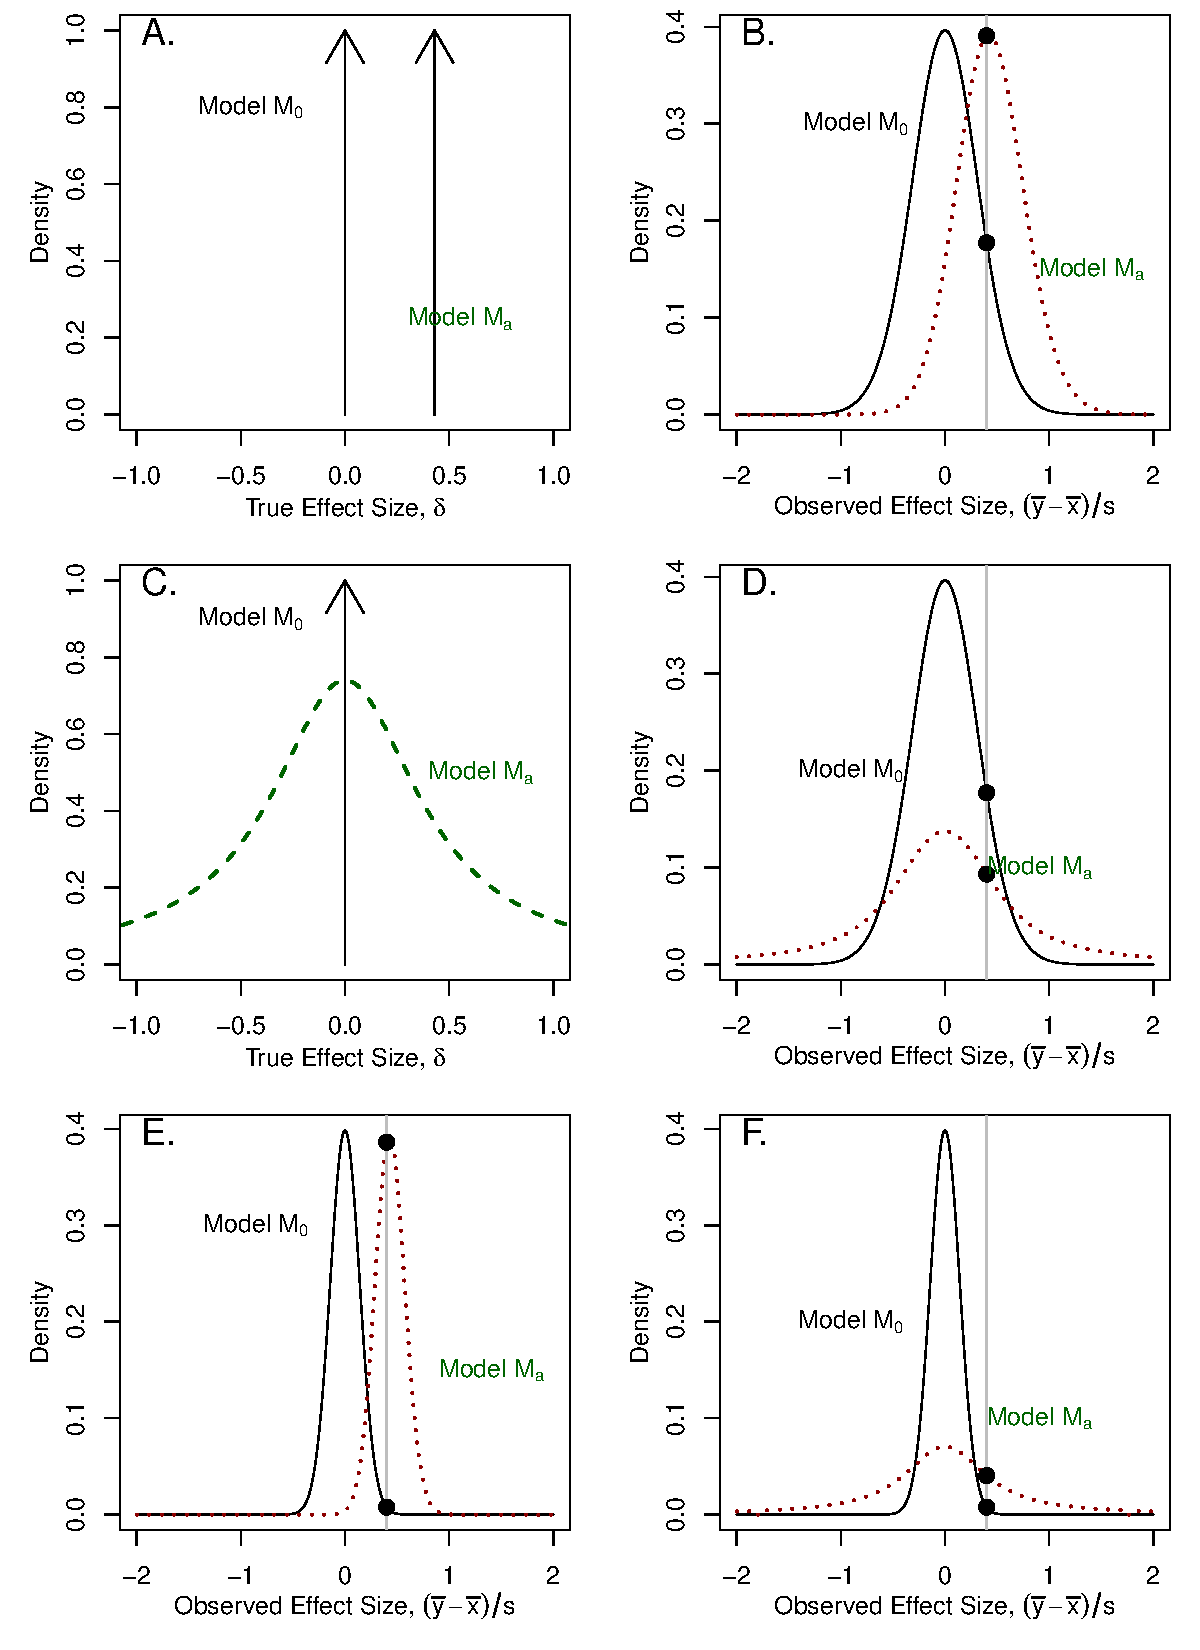
\includegraphics[width=\textwidth, keepaspectratio]{BFfigure.pdf}
\caption{Bayesian model comparison.}
\label{BFfig}
\end{figure}
% image dimensions far exceed table dimensions

\begin{table}
\caption{Pilot test results.}
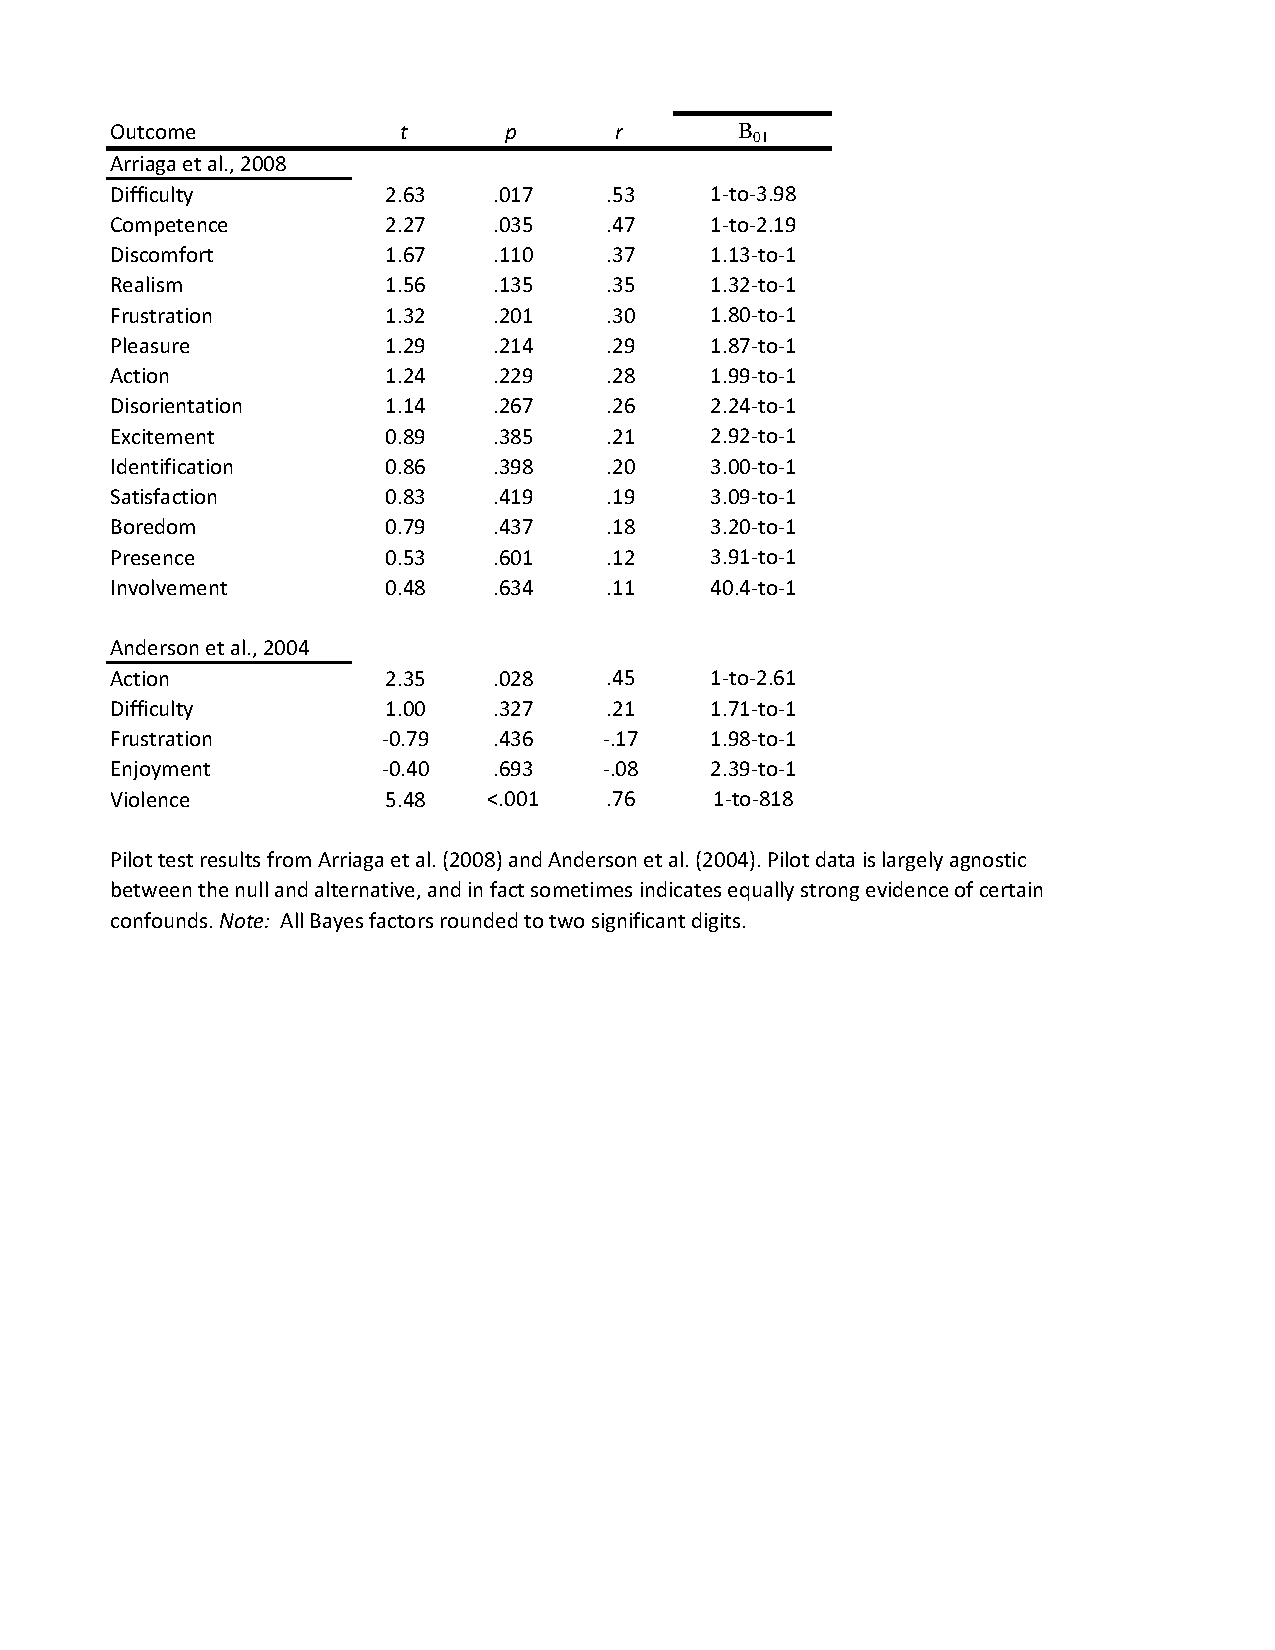
\includegraphics{Arriaga_Anderson_table.pdf}
%\begin{tabular}{lcccc} 
%&$t$&$p$&$r$&$BF_{01}$ \\ \hline
%Arriaga et al., 2008 \\ \cline{1-1}
%Difficulty&2.63&.017&.53&1-to-3.98 \\
%Competence&2.27&.035&.47&1-to-2.19 \\
%Discomfort&1.67&.110&.37&1.13-to-1 \\ 
%Realism&1.56&.135&.35&1.32-to-1 \\
%Frustration&1.32&.201&.30&1.80-to-1 \\
%Pleasure&1.29&.214&.29&1.87-to-1 \\
%Action&1.24&.229&.28&1.99-to-1 \\
%Disorientation&1.14&.267&.26&2.24-to-1 \\ 
%Excitement&0.89&.385&.21&2.92-to-1 \\
%Identification&0.86&.398&.20&3.00-to-1 \\
%Satisfaction&0.83&.419&.19&3.09-to-1 \\ 
%Boredom&0.79&.437&.18&3.20-to-1 \\ 
%Presence&0.53&.601&.12&3.91-to-1 \\
%Involvement&0.48&.634&.11&40.4-to-1 \\
%&&&& \\ 
%Anderson et al., 2004 \\ \cline{1-1}
%Action&2.35&.028&.45&1-to-2.61 \\
%Difficulty&1.00&.327&.21&1.71-to-1 \\
%Frustration&-0.79&.436&-.17&1.98-to-1 \\
%Enjoyment&-0.40&.693&-.08&2.39-to-1 \\
%Violence&5.48&$<.001$&.76&1-to-818 \\
%\multicolumn{5}{l}{\multirow{2}{90mm}{Pilot test results from \citet{Arriaga:etal:2008} and \citet{Anderson:etal:2004}. Pilot data is largely agnostic between the null and alternative, and in fact sometimes indicates equally strong evidence of certain confounds. {\em Note:} $B_{01}$ ranges from 1-to-$\infty$ (perfect evidence for alternative) to $\infty$-to-1 (perfect evidence for null). Contrary to the authors’ original conclusions, the pilot test has some evidence the games differ in feelings of competence, and fairly substantial evidence that they differ in difficulty. $H_0: |\delta| < .1$; $H_1: \delta \sim Cauchy(scale = .5)$. All Bayes factors rounded to two significant digits.}}
%\end{tabular}
\label{ArriagaAndersonPilot}
\end{table}

% Is this table legible?
\begin{table}
\caption{Pilot test from \citet{Valadez:Ferguson:2012}.} 
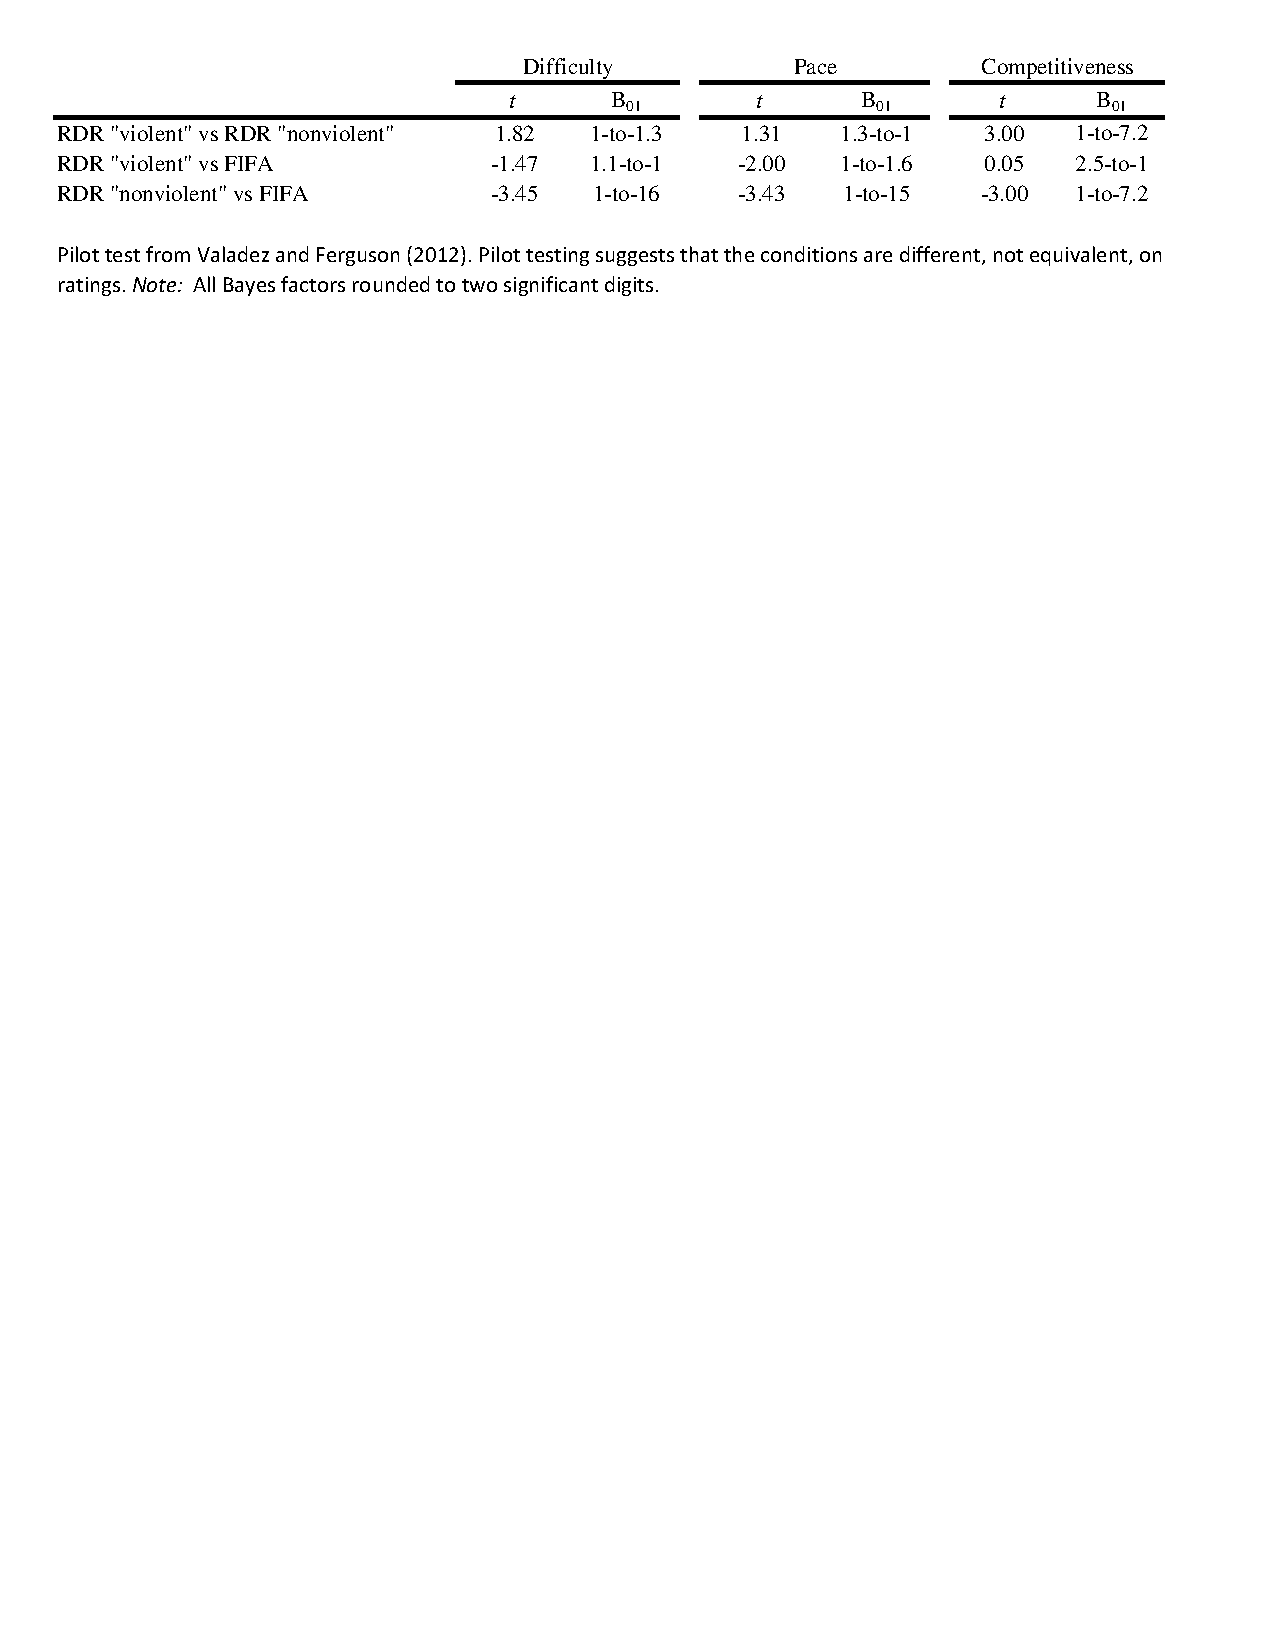
\includegraphics{Valadez_Ferguson_table.pdf}
%Pilot testing suggests that the conditions are different, not equivalent, on ratings. $BF_{01}$ ranges from 1-to-$\infty$ (perfect evidence for alternative) to $\infty$-to-1 (perfect evidence for null). $H_0: \delta \sim \mbox{Uniform[-0.1, 0.1]}$; $H_1: \delta \sim \mbox{Cauchy(scale = .5)}$. All Bayes factors rounded to two significant digits.}
%\begin{tabular}{l@{\hspace{1cm}} cc@{\hspace{1cm}} cc@{\hspace{1cm}} cc}
%& \multicolumn{2}{c}{Difficulty} & \multicolumn{2}{c}{Pace} & \multicolumn{2}{c}{Competitiveness} \\
%\cline{2-3} \cline{4-5} \cline{6-7} 
%& $t$ & $BF_{01}$ & $t$ & $BF_{01}$ & $t$ & $BF_{01}$ \\ \hline
%Active vs. Control1 & 1.82 & 1-to-1.3 & 1.31 & 1.3-to-1 & 3.00 & 1-to-7.2 \\
%Active vs. Control2 & -1.47 & 1.1-to-1 & -2.00 & 1-to-1.6 & 0.05 & 2.5-to-1 \\
%Control1 vs. Control2 & -3.45 & 1-to-16 & -3.43 & 1-to-15 & -3.00 & 1-to-7.2 \\
%\end{tabular}
\label{ValadezFergusonPilot}
\end{table}

\begin{table}
\caption{Bayesian re-analysis of null results.}
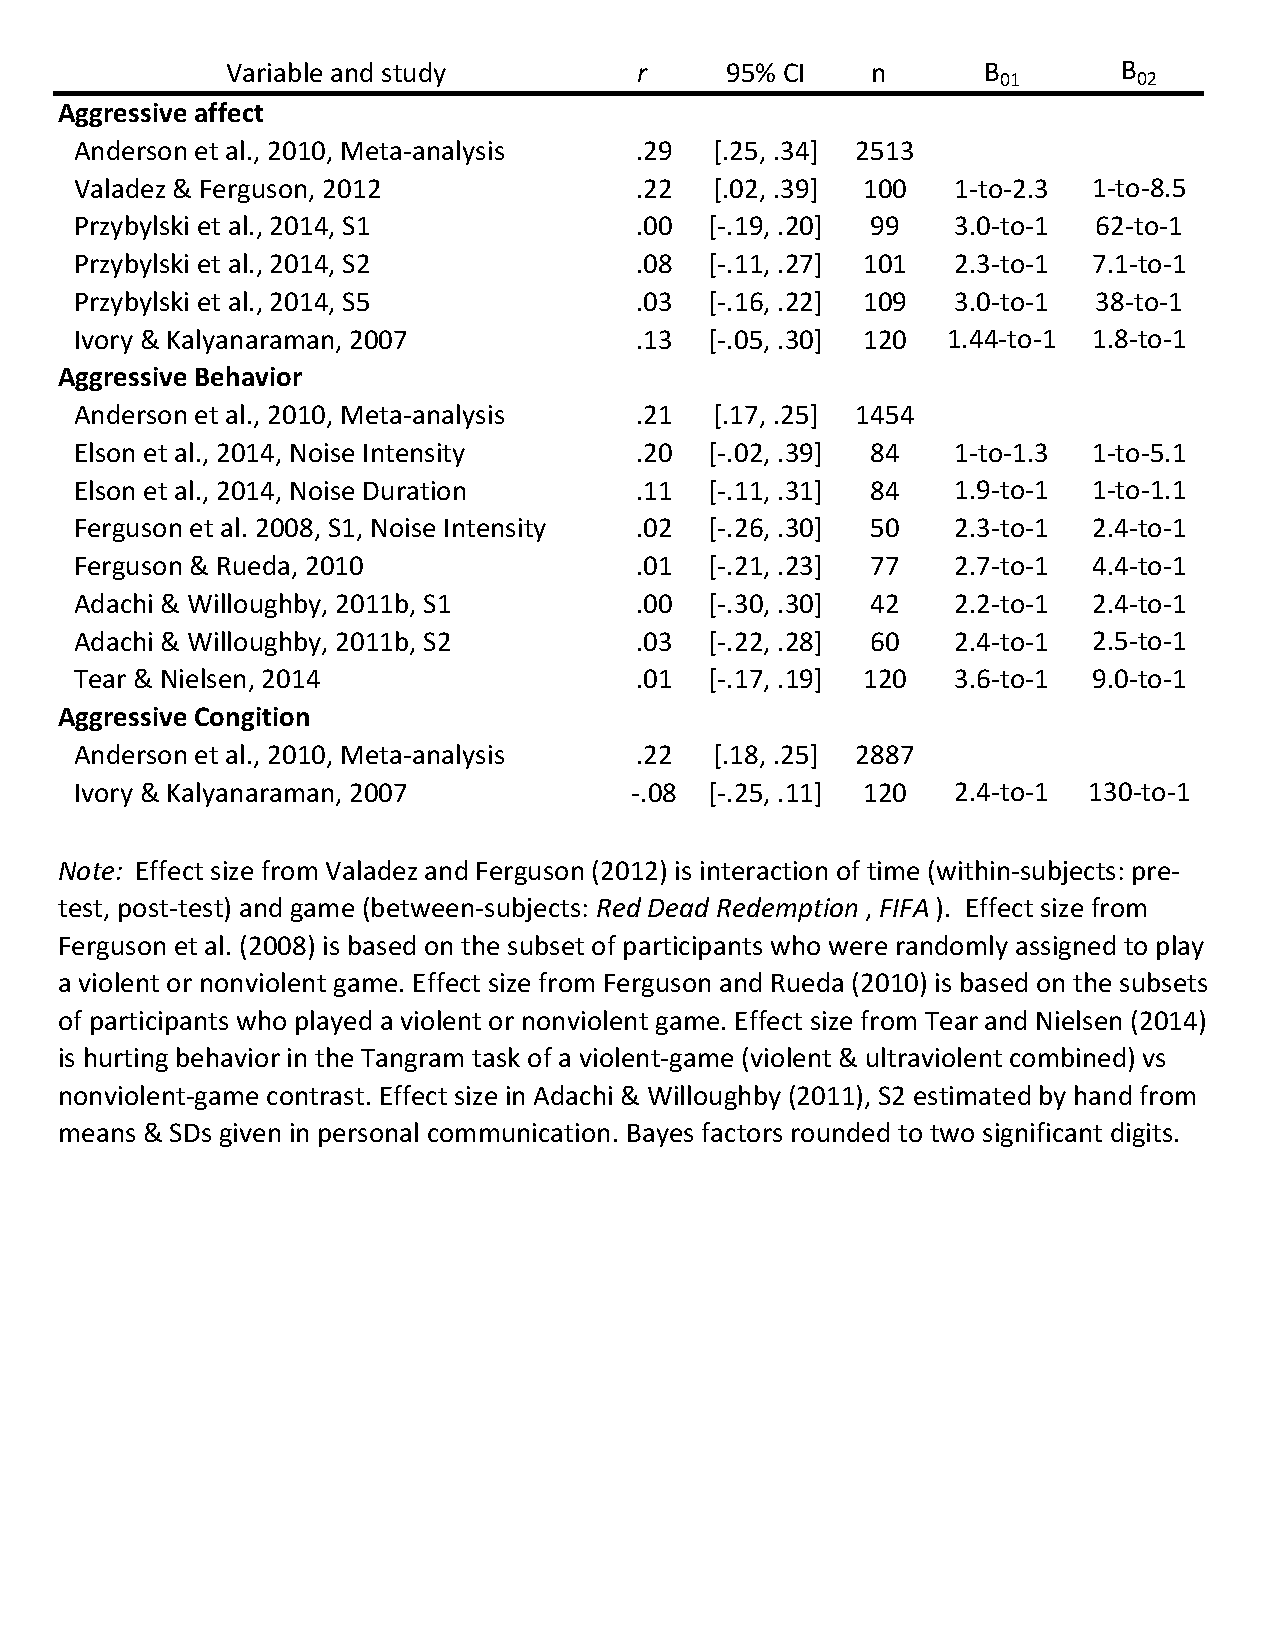
\includegraphics[width=\textwidth, scale=1]{Main Study Results.pdf}
%Some studies present only modest evidence against the effect, and several indicate evidence for the effect despite nonsignificant p-values. $BF_{01}$ = evidence for $H_0: \delta = 0$ compared to $HA_1: \delta \sim$ Cauchy(scale = 0.4). $BF_{02}$ = evidence for $H_0: \rho = 0$ compared to $H_{A2}: \rho \sim \mbox{Normal}(\mu, \sigma)$, with $\mu$ and $\sigma$ taken from \citet{Anderson:etal:2010}. Bayes factors range from 1-to-$\infty$ (perfect evidence for alternative) to $\infty$-to-1 (perfect evidence for null). All Bayes factors rounded to two significant digits.}
%\begin{tabular}{p{8cm}ccccc}
%&r   &95\% CI&n  &$BF_{01}$ & $BF_{02}$ \\
%Aggressive affect&&&&& \\
%Anderson et al., 2010, Meta-analysis&.29&[.25, .34]&2513&& \\
%Valadez \& Ferguson, 2012, interaction effect&.22&[.02, .39]&100&1-to-2.3&1-to-8.5 \\
%Przybylski et al., 2014, Study 1&.00&[-.19, .20]&99&3.0-to-1&62-to-1 \\
%Przybylski et al., 2014, Study 2&.08&[-.11, .27]&101&2.3-to-1&7.1-to-1 \\
%Przybylski et al., 2014, Study 5&.03&[-.16, .22]&109&3.0-to-1&38-to-1 \\
%Ivory \& Kalyanaraman, 2007&.13&[-.05, .30]&120&1.44-to-1&1.8-to-1 \\
%Aggressive Behavior&&&&& \\
%Anderson et al., 2010, Meta-analysis&.21&[.17, .25]&1454&& \\
%Elson et al., 2014, Noise Intensity&.20&[-.02, .39]&84&1-to-1.3&1-to-5.1 \\
%Elson et al., 2014, Noise Duration&.11&[-.11, .31]&84&1.9-to-1&1-to-1.1 \\
%Ferguson et al. 2008, Study 1 – Random assignment, Noise Intensity&.02&[-.26, .30]&50&2.3-to-1&2.4-to-1 \\
%Ferguson \& Rueda, 2010 – Violent vs. nonviolent game&.01&[-.21, .23]&77&2.7-to-1&4.4-to-1 \\
%Adachi \& Willoughby, 2011b, Experiment 1&.00&[-.30, .30]&42&2.2-to-1&2.4-to-1 \\
%Adachi \& Willoughby, 2011b, Experiment 2&.03&[-.22, .28]&60&2.4-to-1&2.5-to-1 \\
%Tear \& Nielsen, 2014, hurting behavior in Tangram task&.01&[-.17, .19]&120&3.6-to-1&9.0-to-1 \\
%Aggressive Cognition&&&&& \\
%Anderson et al., 2010, Meta-analysis&.22&[.18, .25]&2887&& \\
%Ivory \& Kalyanaraman, 2007&-.08&[-.25, .11]&120&2.4-to-1&130-to-1 \\
%\end{tabular}
\label{mainStudyResults}
\end{table}

\begin{table}
\caption{Bayes factors for each effect size as calculated by \citet[study 2, table 2]{Elson:etal:2014}.}
\centering
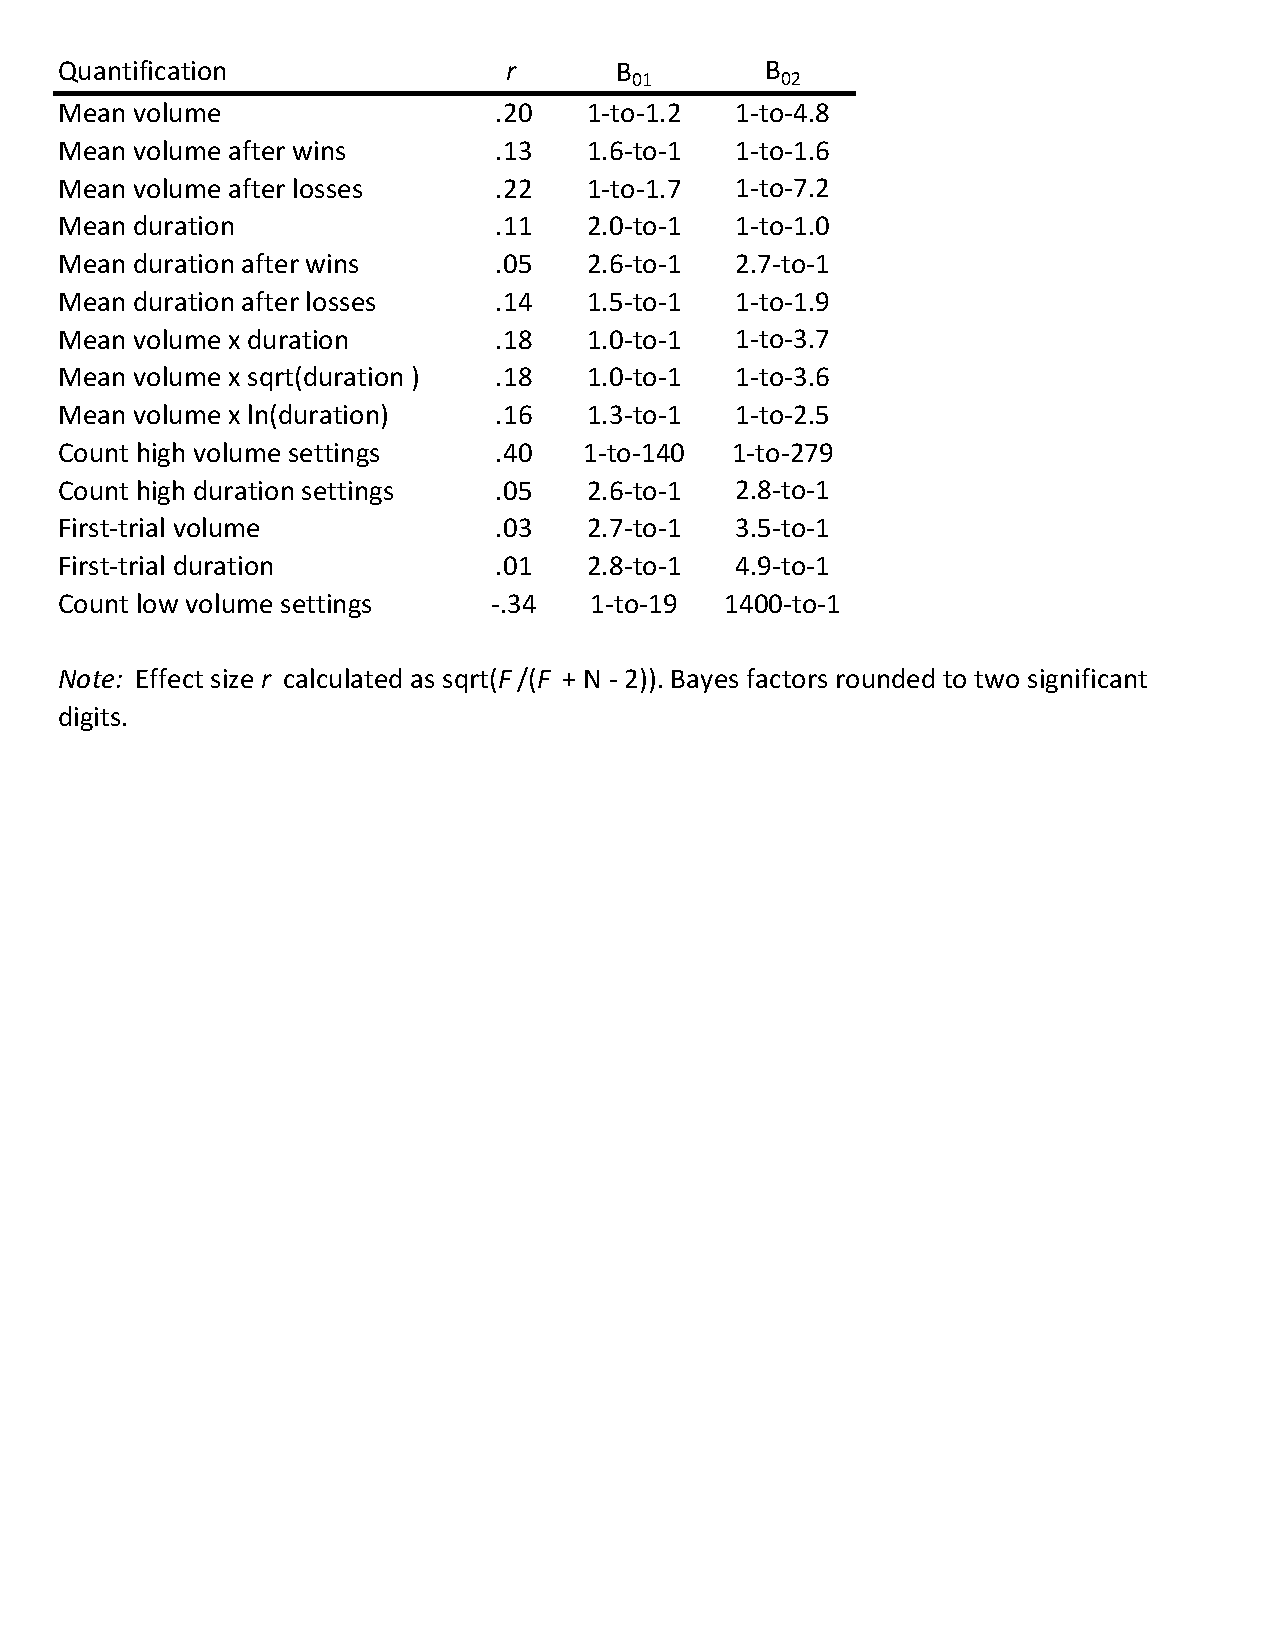
\includegraphics[width=\textwidth, scale=2]{Elson_CRTT-hacking.pdf}
%\begin{tabular}{lccc}
%Quantification&r&$BF_{01}$&$BF_{02}$ \\ \hline
%Mean volume&.20&1-to-1.2&1-to-4.8 \\
%Mean volume after wins&.13&1.6-to-1&1-to-1.6 \\
%Mean volume after losses &.22&1-to-1.7&1-to-7.2 \\
%Mean duration &.11&2.0-to-1&1-to-1.0 \\
%Mean duration after wins&.05&2.6-to-1&2.7-to-1 \\
%Mean duration after losses &.14&1.5-to-1&1-to-1.9 \\
%Mean volume x duration &.18&1.0-to-1&1-to-3.7 \\
%Mean volume x sqrt(duration)&.18&1.0-to-1&1-to-3.6 \\
%Mean volume x ln(duration) &.16&1.3-to-1&1-to-2.5 \\ 
%Count high volume settings &.40&1-to-140&1-to-279 \\
%Count high duration settings &.05&2.6-to-1&2.8-to-1 \\
%First-trial volume &.03&2.7-to-1&3.5-to-1 \\ 
%First-trial duration&.01&2.8-to-1&4.9-to-1 \\
%Count low volume settings&-.34&1-to-19&1400-to-1 \\
%\end{tabular}
\label{ElsonCRTTHacking}
\end{table}

\newpage
\bibliography{database}
\end{document}